\documentclass[t,9pt,svgnames]{beamer}
\usepackage[latin1]{inputenc}
\usepackage{framed}
\usepackage{graphics}
\usepackage{helvet}
\usepackage{courier}
\usepackage{amsmath}
\usepackage[absolute,overlay]{textpos}
\usepackage{fancybox}
%\usepackage{color}
\usepackage{bm} % Use \bm to generate bold math fonts

%%%%% NOTE TO USER %%%%%%%
%
%  This template requires the 'frame-bg.pdf' and 'title-bg.pdf' be found.  It should have been included with
%  this example.
%%%%%%%%%%%%%%%%%%%%%%%%%

\graphicspath{
{graphics/}
}

\usetheme{INL}

\usepackage{listings}
\lstset{
  basicstyle=\ttfamily\scriptsize,
  frame=single,
  backgroundcolor=\color{cbbkng},
  emphstyle={\color{red}\textbf},
	showstringspaces=false,
  commentstyle=\color{inl@green},
	keywordstyle=\bfseries,
  escapeinside=$$
}

\setbeamercolor{codeboxcolor}{fg=white,bg=black}

\definecolor{bubblebkng}{rgb}{0.98,0.98,0}
%\definecolor{cbbkng}{rgb}{0.98,0.9,0.98}
\definecolor{cbbkng}{RGB}{227,233,252}

\newenvironment{codebox}{}{}
% #1 - width
% #2 - position on the page (<dim>,<dim>)
% #3 - text
\newcommand{\bubbleat}[3]{\begin{textblock*}{#1}[1,1](#2)
\fcolorbox{black}{yellow}{%
\scriptsize\begin{Bcenter}
#3
\end{Bcenter}}
\end{textblock*}}

\newcommand{\uo}{\ensuremath{\mbox{UO}_2}}
\newcommand{\mytilde}{\raise.17ex\hbox{$\scriptstyle\sim$}}

\newcommand{\code}[1]{\texttt{#1}}
\newcommand{\comment}[1]{{\usebeamercolor[fg]{comment code} #1}}

\newenvironment{codelst}{\begin{verbatim}}{\end{verbatim}}

\newcommand{\blue}[1]{{\color{blue}#1}}
\newcommand{\red}[1]{{\color{red}#1}}

% TOC
\newdimen\tocpnumwd
\tocpnumwd=30pt

\makeatletter

\def\dottedtocline#1#2#3{\bgroup%
  \advance\leftskip by #1%
  \advance\rightskip by #2%
  \advance\rightskip by \tocpnumwd%
  \leaders\hbox to 1.5em{\hss .\hss}\hfill\nobreak%
  \rlap{\hbox to \tocpnumwd{\hfil #3}}\par\egroup}

%\def\beamer@sectionintoc #1#2#3#4#5{{\small#2\dottedtocline{7em}{6em}{#3}}\par}
\def\beamer@sectionintoc #1#2#3#4#5{{\hspace{5em}\hyperlink{Navigation#3}{\small#2\dotfill{#3}}\hspace*{4em}}\par}


%\def\beamer@subsectionintoc %#1#2#3#4#5#6{{\small#3\dottedtocline{9em}{6em}{#4}}\par}
\def\beamer@subsectionintoc #1#2#3#4#5#6{{\hspace{6em}\hyperlink{Navigation#4}{\small#3\dotfill{#4}}\hspace*{4em}}\par}

\newcommand{\mytoc}{\@starttoc{toc}}

\makeatother

%This is an ugly hack to fix a bug with Beamer that doesn't put enough vertical
%space above the first list environment in a columns environment when the [t]
%option is passed to the beamer class.  Use this command somewhere in the
%column before using a list or itemize
\newcommand{\vspacehack}{
\setbox0=\vbox{
\begin{itemize}
\item
\end{itemize}
}}


\begin{document}

% user start editing here! %
\title[RAVEN Workshop]{RAVEN Workshop}
\subtitle{Multi-Step Input Space Reduction}
\institute[INL]{Nuclear Engineering Methods Development Department\\
Idaho National Laboratory}

\begin{titleframe}{RAVEN Workshop}

{\bfseries\emph{Multi-Step Input Reduction}}

\vfill
{\small Nuclear Engineering Methods Development Department\\
Idaho National Laboratory}
\end{titleframe}

\begin{frame}{Discussion Points}
\mytoc
\end{frame}

%                  %
%     OVERVIEW     %
%                  %
\section{Overview}
\begin{frame}{Overview}
\end{frame}

\begin{frame}{Overview: Uncertainty Quantification}
  \vfill
  Benefits:
  \vfill
  \begin{itemize}
    \item Quantity of Interest Variance
  \vfill
    \item Failure Probabilities
  \vfill
    \item Limit Surface Construction
  \vfill
    \item Design of Experiment
  \end{itemize}
  \vfill
\end{frame}

\begin{frame}{Overview: Session Goal}
  \vfill
  Reduce high-dimension input spaces
  \vfill
  \begin{itemize}
    \item Use PCA to eliminate correlated inputs
  \vfill
    \item Use sensitivity to eliminate low-impact inputs
  \vfill
    \item Accurate UQ on a reduced input space
  \end{itemize}
  \vfill
\end{frame}

\begin{frame}{Overview: Assumptions}
  We assume:
  \vfill
  \begin{itemize}
    \item Simulation codes are expensive to run
  \vfill
    \item All inputs are initially perturbable
  \vfill
    \item Saving time and money is good
  \end{itemize}
  \vfill
\end{frame}

%                  %
%    MOTIVATIONS   %
%                  %
\section{Motivations}
\begin{frame}{Motivations}
\end{frame}

\begin{frame}{Motivations: Sampling Strategies}
  \vfill
  Two classes of forward sampling strategies in RAVEN:
  \begin{columns}
    \begin{column}{0.5\textwidth}
      \vspacehack
      ~\\~\\
      ~\\
      \begin{itemize}
        \item Structured (Orthogonal Grids, Limit Surface, Latin Hypercube)
      ~\\~\\~\\
      ~\\~\\~\\~\\
        \vfill
        \item Unstructured (Monte Carlo)
      \end{itemize}
      \vfill
    \end{column}
    \begin{column}{0.5\textwidth}
      \begin{figure}
        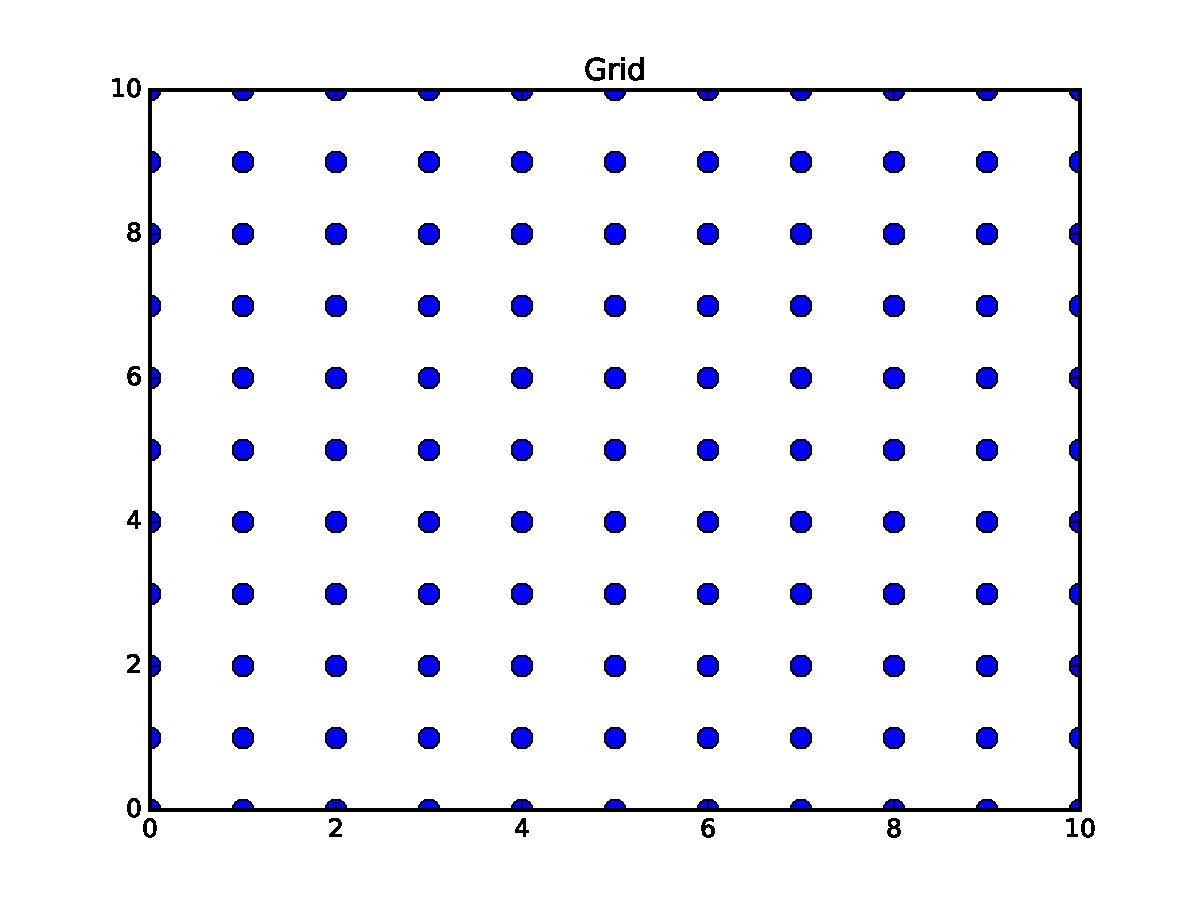
\includegraphics[width=0.7\linewidth]{pics/grid.pdf}
      \end{figure}
      \begin{figure}
        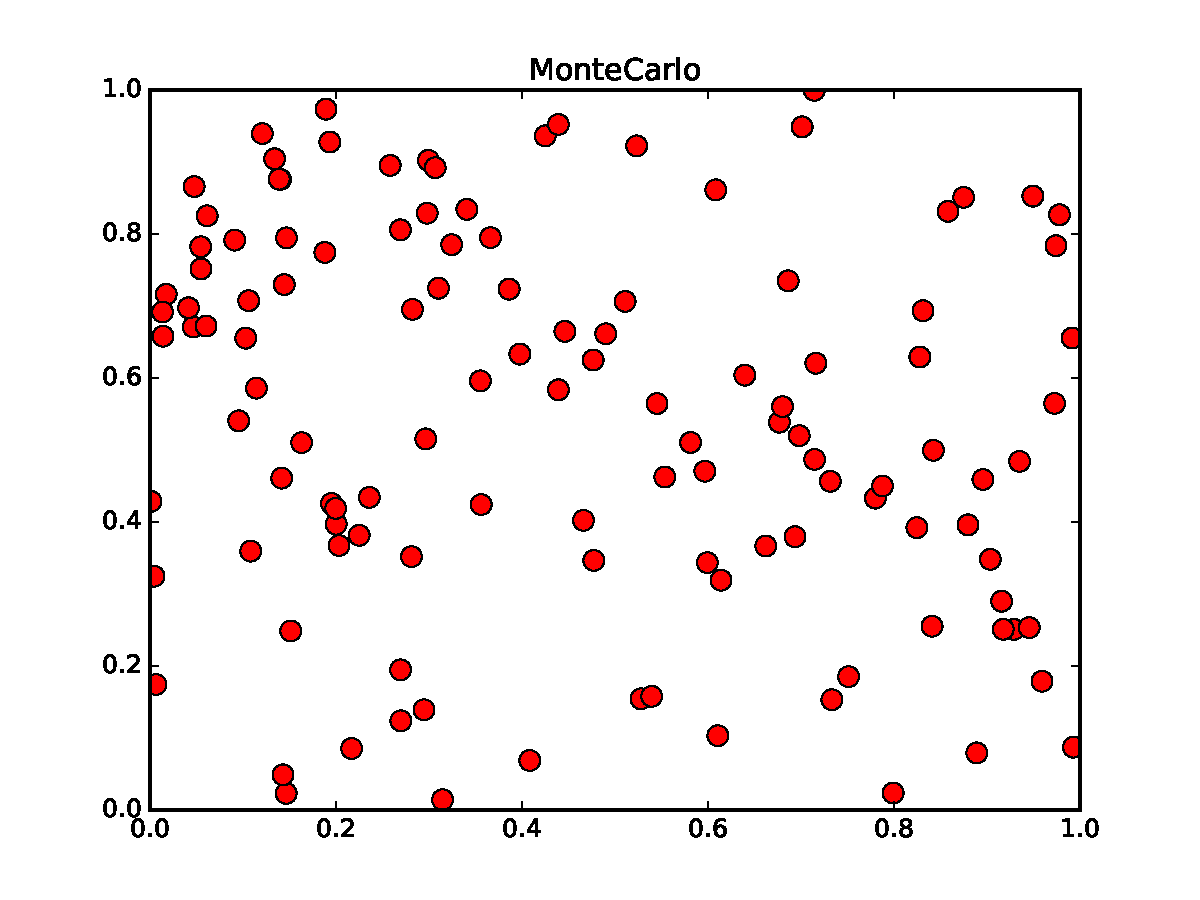
\includegraphics[width=0.7\linewidth]{pics/mc.pdf}
      \end{figure}
    \end{column}
  \end{columns}
  \vfill
\end{frame}

\begin{frame}{Motivations: Unstructured Sampling}
  \vfill
  \begin{columns}
    \begin{column}{0.5\textwidth}
      ~\\~\\
      Traditional Monte Carlo sampling
      ~\\~\\
      \begin{itemize}
        \item Agnostic of Dimensionality
      ~\\~\\
        \item Consistent, but slow convergence
      \end{itemize}
      ~\\~\\
    \end{column}
    \begin{column}{0.5\textwidth}
      \begin{figure}
        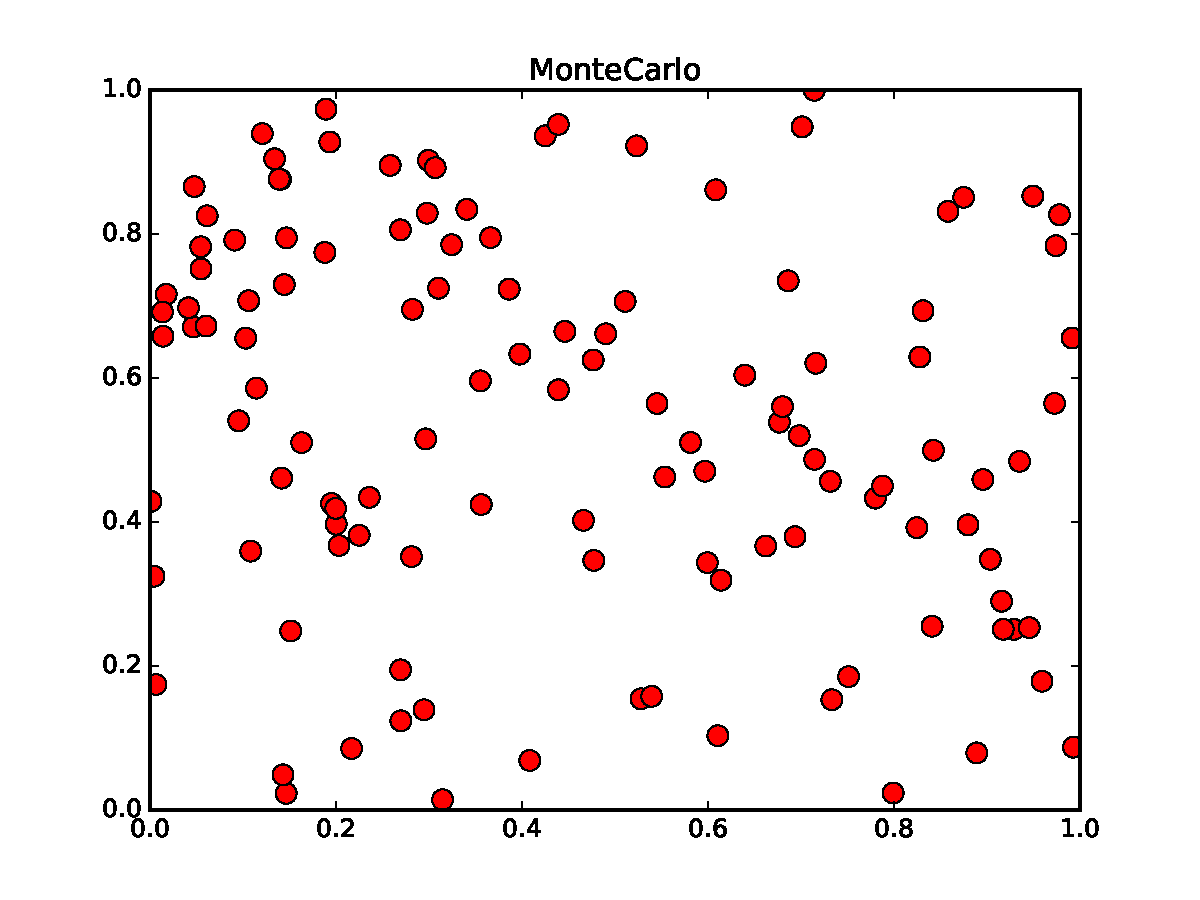
\includegraphics[width=\linewidth]{pics/mc.pdf}
      \end{figure}
    \end{column}
  \end{columns}
  \vfill
\end{frame}

\begin{frame}{Motivations: Structured Sampling}
  \vfill
  \code{RAVEN} has several structured solvers
  \begin{columns}
    \begin{column}{0.5\textwidth}
      ~\\~\\
      \begin{itemize}
        \item Orthogonal Grids
      ~\\~\\~\\
        \item Sparse Grid
      ~\\~\\~\\
        \item Stratified
      ~\\~\\~\\
        \item Limit Surface Search
      \end{itemize}
      ~\\~\\
      All of these suffer from the Curse of Dimensionality
    \end{column}
    \begin{column}{0.5\textwidth}
      \begin{figure}
        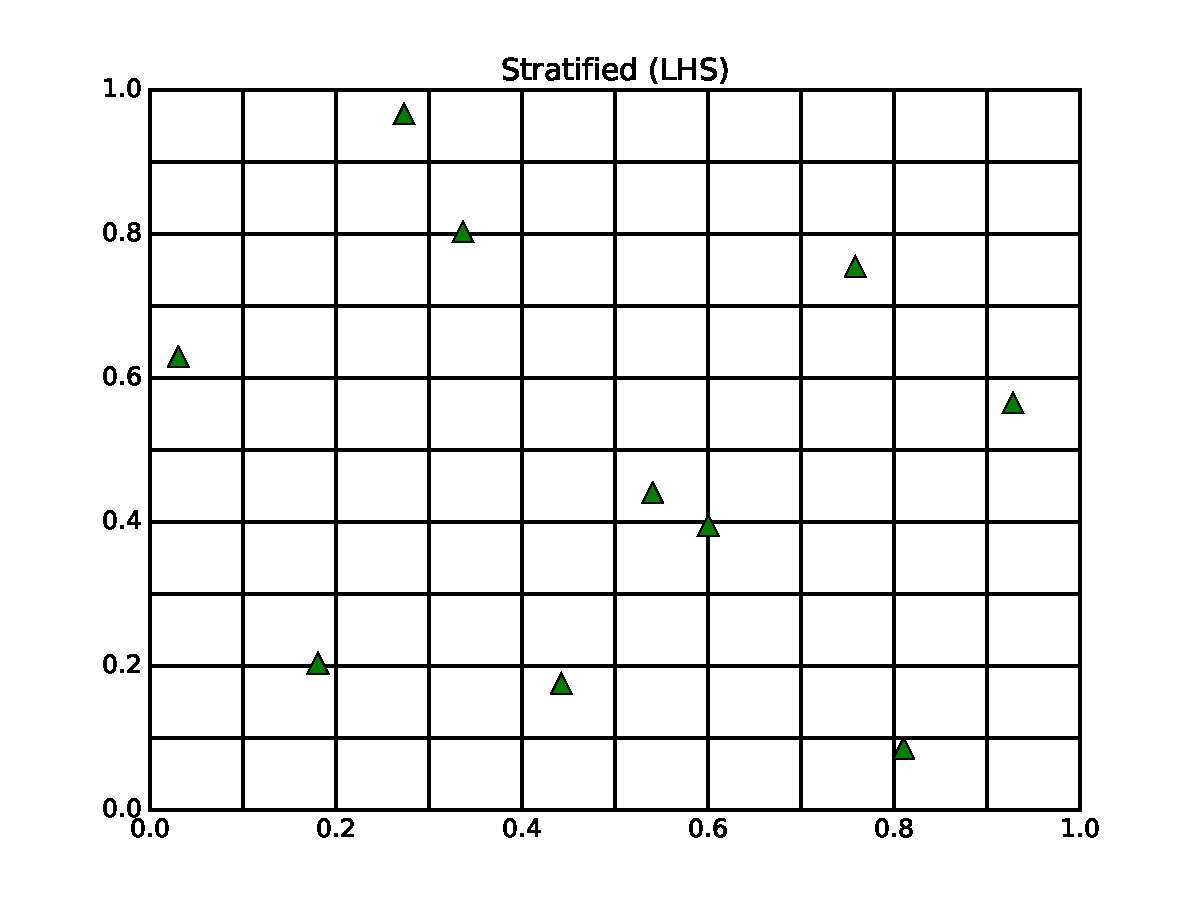
\includegraphics[width=0.7\linewidth]{pics/lhs.pdf}
      \end{figure}
      \begin{figure}
        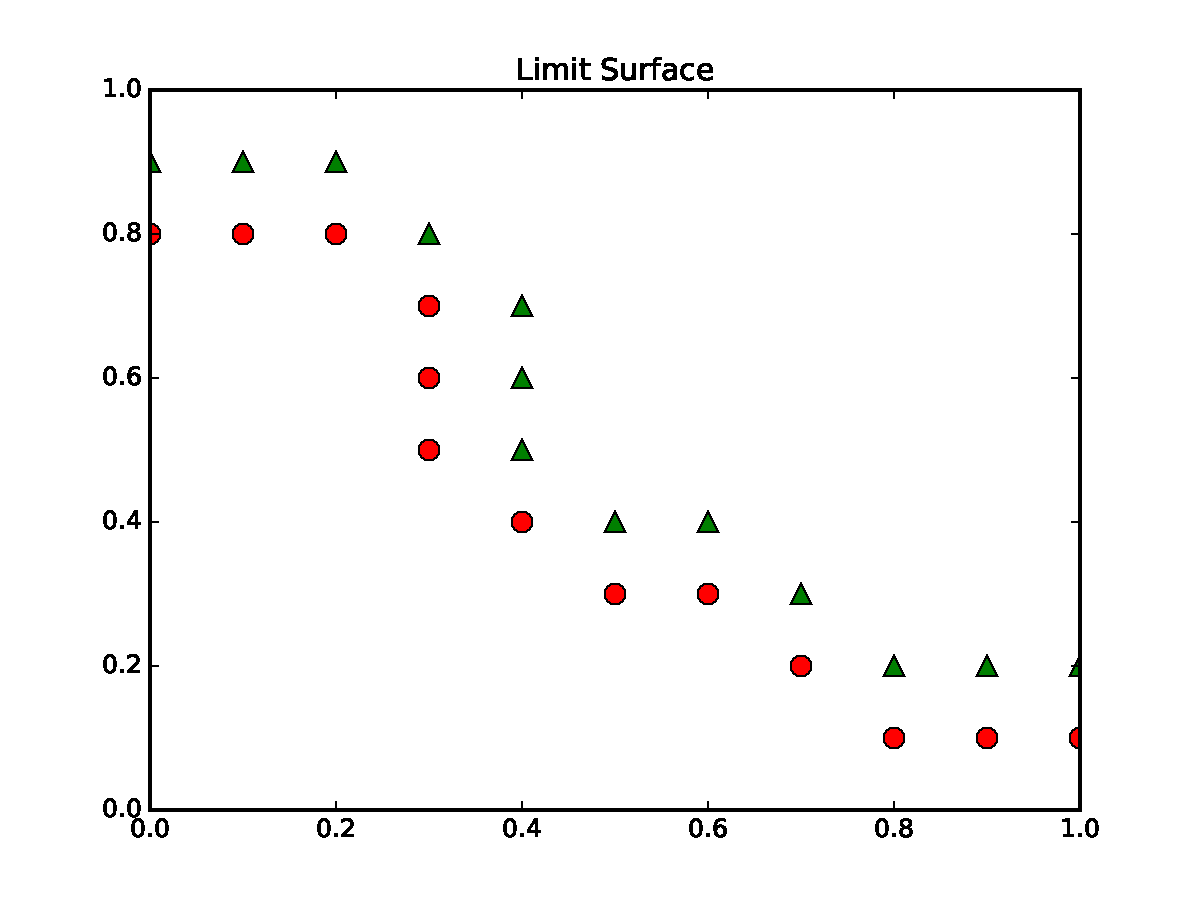
\includegraphics[width=0.7\linewidth]{pics/limit.pdf}
      \end{figure}
    \end{column}
  \end{columns}
  \vfill
\end{frame}

\begin{frame}{Motivations: Proposed Solution}
  \vfill
  Remove unnecessary input dimensions
  \vfill
  \begin{itemize}
    \item Correlated inputs have redundancy
  \vfill
    \item Low-impact inputs aren't useful to perturb
  \end{itemize}
  \vfill
  Perform UQ on reduced space
  \vfill
\end{frame}
%                  %
%      METHODS     %
%                  %
\section{Methods}
\begin{frame}{Methods}
\end{frame}

\begin{frame}{Methods: Procedure Overview}
  \vfill
  \begin{itemize}
    \item (optional) Benchmark original problem
  \vfill
    \item Perform PCA on original input space
  \vfill
    \item Truncate to essential latent variables
  \vfill
    \item Perform global sensitivity analysis
  \vfill
    \item Truncate latent variables to exclude non-essential
  \end{itemize}
\end{frame}
  \vfill

\subsection{Principle Component Analysis}
\begin{frame}{Methods: Principal Component Analysis}
\end{frame}

\begin{frame}{Methods: Principal Component Analysis}
  \vfill
  Used to orthogonalize input space
  \vfill

  Represent input space as sum of ``latent'' variables $\bm{L}$
  \begin{equation}
    \bm{M} = \bm{Q} \cdot \bm{L},
  \end{equation}
  where
  \vfill
  \begin{itemize}
    \item $\bm{M}$ is the vector of original variables, $|M|\times1$,
  \vfill
    \item $\bm{Q}$ is the PCA transformation matrix, $|M|\times |L|$,
  \vfill
    \item $\bm{L}$ is the vector of latent variables, $|L|\times 1$
  \end{itemize}
  \vfill
  All $\bm{L}$ are distributed as standard normal distributions
  \vfill
\end{frame}

\begin{frame}{Methods: Principal Component Analysis}
  \vfill
  \begin{equation}
    \bm{M} = \bm{Q} \cdot \bm{L},
  \end{equation}
  \vfill
  Perform eigenvalue decomposition of covariance matrix and rank eigenvalues
  \vfill

  Truncate latent variables at desirable eigenvalue
  \vfill
      \begin{figure}
        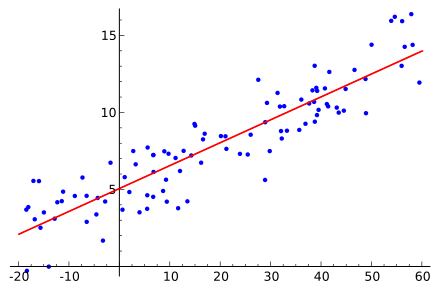
\includegraphics[width=0.4\linewidth]{pics/pca.png}
      \end{figure}
  \vfill
  %TODO show list and truncation pic
\end{frame}

\begin{frame}[fragile]{Methods: PCA in RAVEN}
  \vfill
Add transformation to \code{Sampler}:
\lstinputlisting[firstline=41,lastline=68,emph={variablesTransformation,x1,x2,x3,x4,x5,x6,y1,y2,y3,y4,y5,y6}]{../../inputs/two-step-input-reduction/wk_example/mc_pca.xml}
  \vfill
\end{frame}

\begin{frame}[fragile]{Methods: PCA in RAVEN}
  \vfill
  Use a PostProcessor to extract the rankings
  \vfill

  PostProcessor
\lstinputlisting[firstline=17,lastline=23,emph={ImportanceRank,stats,pcaindex,y1,y2,y3,y4,y5,y6,ans,mvn}]{../../inputs/two-step-input-reduction/wk_example/mc_pca.xml}
  \vfill
  Step
\lstinputlisting[firstline=82,lastline=86,emph={stats,solns,statsfile}]{../../inputs/two-step-input-reduction/wk_example/mc_pca.xml}
  \vfill
Use results from file TODO to pick PCA truncation
  \vfill
\end{frame}

\begin{frame}[fragile]{Methods: PCA in RAVEN}
  \vfill
  Once reduction level is decided, change sampler truncation and distribution truncation
  \lstinputlisting[firstline=40,lastline=59,emph={y1,y2,y3,y4}]{../../inputs/two-step-input-reduction/wk_example/sobol_sens.xml}
  \vfill
\end{frame}

\begin{frame}[fragile]{Methods: PCA in RAVEN}
  \vfill
  Once reduction level is decided, change sampler truncation and distribution truncation
  \lstinputlisting[firstline=23,lastline=36,emph={transformation,rank}]{../../inputs/two-step-input-reduction/wk_example/sobol_sens.xml}
  \vfill
\end{frame}


\subsection{Global Sensitivity Analysis}
\begin{frame}{Methods: Global Sensitivity Analysis}
\end{frame}

\begin{frame}{Methods: Global Sensitivity Analysis}
  \vfill
  Now that we've reduced the input, we can do global sensitivity analysis
  \vfill
  \begin{itemize}
    \item Pearson Correlation Coefficients
  \vfill
    \item Spearman Rank Coefficients
  \vfill
    \item Sobol Sensitivity Coefficients
  \end{itemize}
  \vfill
  Pearson and Spearman can be sampled using forward samplers
  \vfill

  Linear Sobol expansion often more efficient (1 run per latent variable)
  \vfill
\end{frame}

\begin{frame}{Methods: Global Sensitivity Analysis}
  \vfill
  Pearson Coefficients
  \vfill
  \begin{itemize}
    \item Global correlation between dimensions
  \vfill
    \item Can be input-input, input-output, or output-output
  \vfill
    \item Can be calculated using most RAVEN Samplers
  \end{itemize}
  \vfill
  %TODO add picture
\end{frame}

\begin{frame}[fragile]{Methods: Global Sensitivity Analysis}
  \vfill
  More on Sobol sampler and HDMRRom in Collocation workshop!
  \vfill

  Sobol sampler
  \lstinputlisting[firstline=40,lastline=59,emph={Sobol,sobolsamp,ROM,rom}]{../../inputs/two-step-input-reduction/wk_example/sobol_sens.xml}
  \vfill
\end{frame}

\begin{frame}[fragile]{Methods: Global Sensitivity Analysis}
  \vfill
  HDMRRom
  \lstinputlisting[firstline=13,lastline=19,emph={HDMRRom,SobolOrder}]{../../inputs/two-step-input-reduction/wk_example/sobol_sens.xml}
  \vfill
  ROM Output
  \lstinputlisting[firstline=88,lastline=92,emph={Print,rom}]{../../inputs/two-step-input-reduction/wk_example/sobol_sens.xml}
  \vfill
\end{frame}

\begin{frame}[fragile]{Methods: Global Sensitivity Analysis}
  \vfill
  Steps
  \lstinputlisting[firstline=62,lastline=81,emph={atten,sobolsamp,solns,solns\_dump\_sobol,rom,sobol\_stats,MultiRun,RomTrainer,IOStep}]{../../inputs/two-step-input-reduction/wk_example/sobol_sens.xml}
  \vfill
\end{frame}

\begin{frame}[fragile]{Methods: Global Sensitivity Analysis}
  \vfill
  Output from ROM
  \lstinputlisting[firstline=1,lastline=26,emph={indices,Sobol\_index}]{../../inputs/two-step-input-reduction/wk_example/run/sobol_stats.xml}
  \vfill
\end{frame}

\subsection{Twice-Reduced Space}
\begin{frame}[fragile]{Methods: Twice-Reduced Analysis}
  \vfill
  Change dimensions in Sampler to prioritize
  \lstinputlisting[firstline=37,lastline=55,emph={y1,y2,y4}]{../../inputs/two-step-input-reduction/wk_example/mc_twice.xml}
  \vfill
\end{frame}

\begin{frame}[fragile]{Methods: Twice-Reduced Analysis}
  \vfill
  Now what?
  \vfill
  \begin{itemize}
    \item Make a ROM
  \vfill
    \item Perform surrogate statistics sampling
  \vfill
    \item Compute limit surface on surrogate
  \end{itemize}
  \vfill
\end{frame}

\section{Full Example}
\begin{frame}[fragile]{Full Example}
  \vfill
  Example case: Cross Section Model
  \vfill
  \begin{itemize}
    \item 308 Correlated Cross Sections (SCALE)
  \vfill
    \item Simulation model is polynomial combinations
  \vfill
    \item PCA Reduction: 308 to 50
  \vfill
    \item Sensitivity Reduction: 50 to 9
  \end{itemize}
  \vfill
  See included examples:
  \vfill
  \begin{itemize}
    \item Original Monte Carlo benchmark: \code{run\char`_mc\char`_orig.xml}
  \vfill
    \item PCA reduction: \code{run\char`_mc\char`_pca.xml}
  \vfill
    \item PCA output: \code{first/TODO}
  \vfill
    \item Sensitivity reduction: \code{run\char`_mc2\char`_[\#].xml}
  \vfill
    \item Sensitivity output: \code{first/sobol\char`_dump.xml}
  \vfill
    \item ROM with twice-reduced space: \code{sc\char`_td[\#].xml}
  \vfill
    \item Twice-reduced output: \code{td\char`_[\#]\char`_dump.xml}
  \end{itemize}
  \vfill
\end{frame}

\begin{frame}[fragile]{Full Example: Mean Results}
  \color{black} Original,
  \color{blue} PCA (50 terms),
  \color{red} PCA (no sens.),
  \color{ForestGreen} PCA and Sensitivity
  \begin{columns}
    \begin{column}{0.5\textwidth}
      \begin{figure}
        \centering
        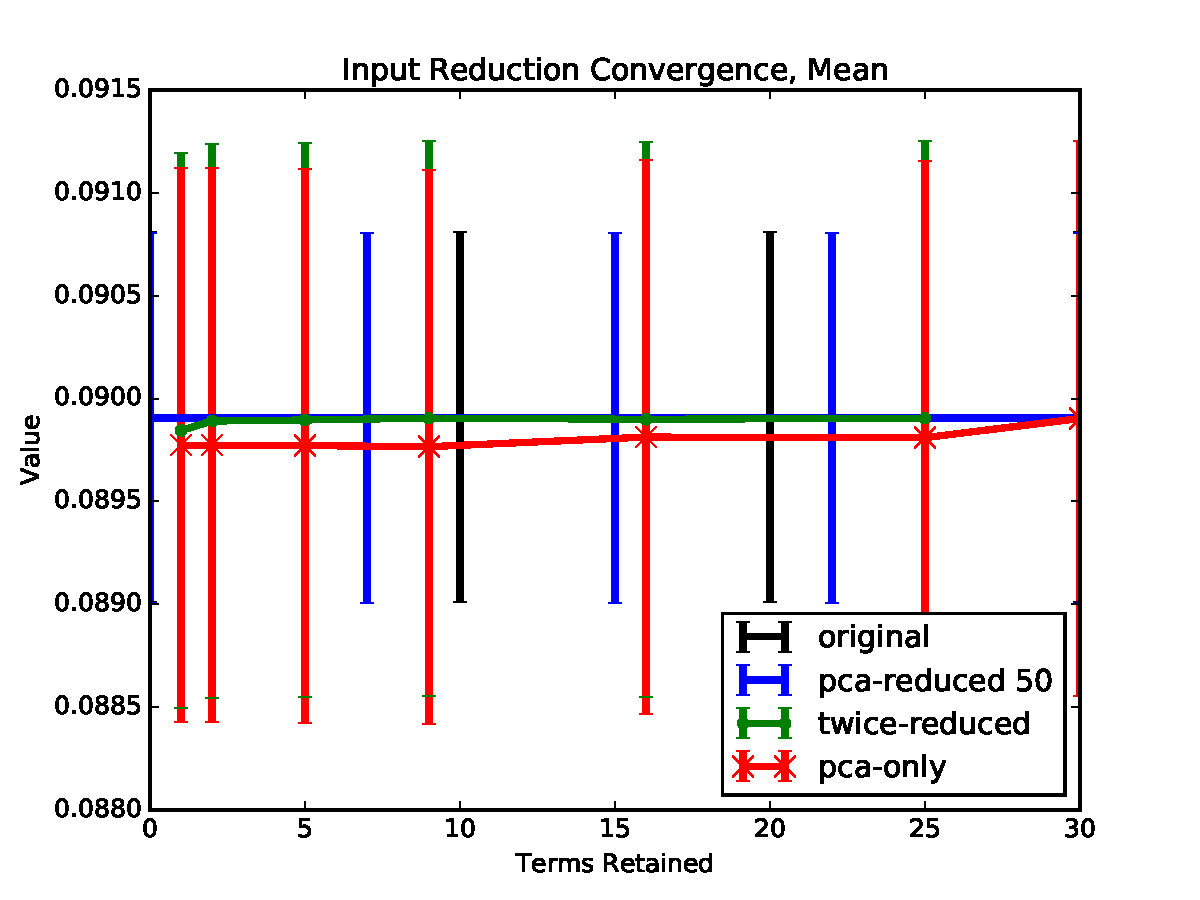
\includegraphics[width=\linewidth]{./example/first/mean.pdf}
        \caption{Mean Values by Terms Kept}
      \end{figure}
    \end{column}
    \begin{column}{0.5\textwidth}
      \begin{figure}
        \centering
        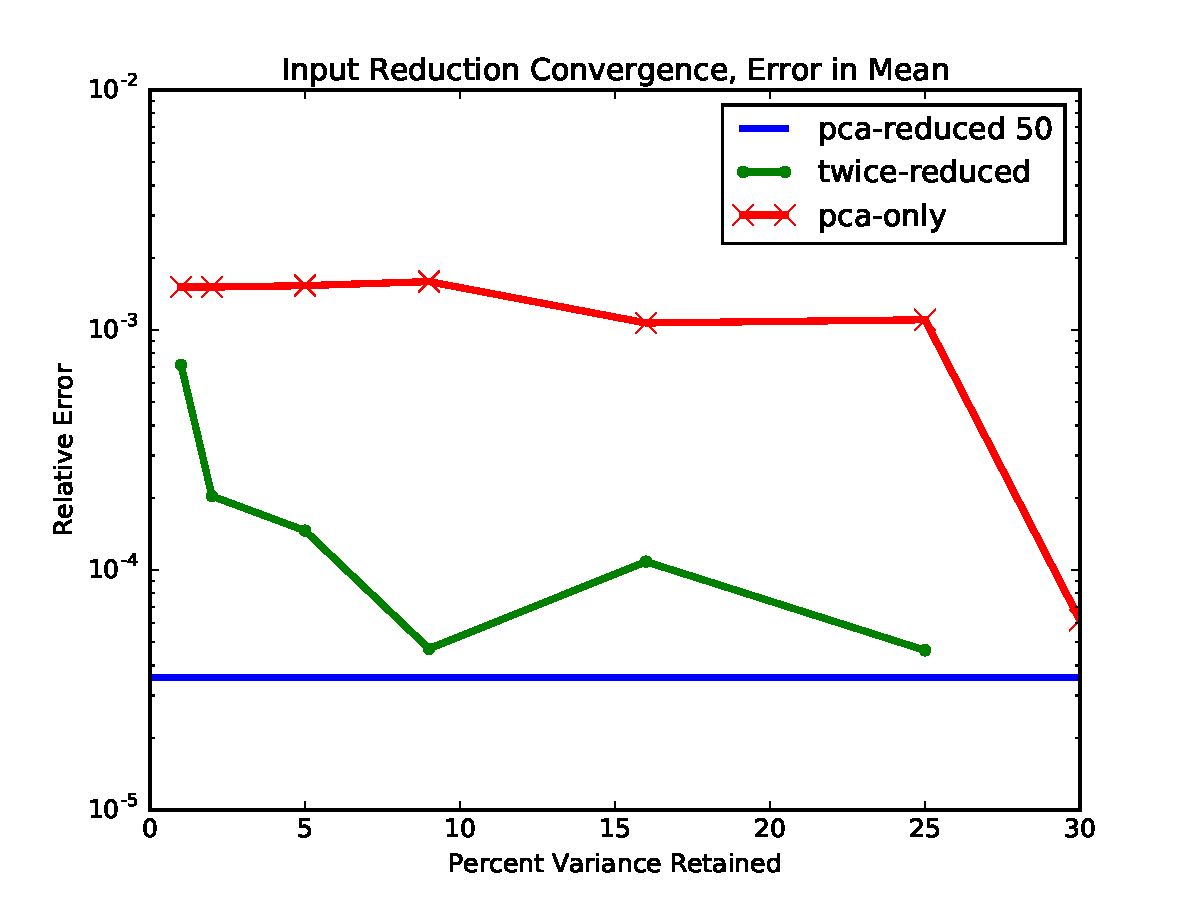
\includegraphics[width=\linewidth]{./example/first/mean_err.pdf}
        \caption{Mean Errors by Terms Kept}
      \end{figure}
    \end{column}
  \end{columns}
\end{frame}

\begin{frame}[fragile]{Full Example: Variance Results}
  \color{black} Original,
  \color{blue} PCA (50 terms),
  \color{red} PCA (no sens.),
  \color{ForestGreen} PCA and Sensitivity
  \begin{columns}
    \begin{column}{0.5\textwidth}
      \begin{figure}
        \centering
        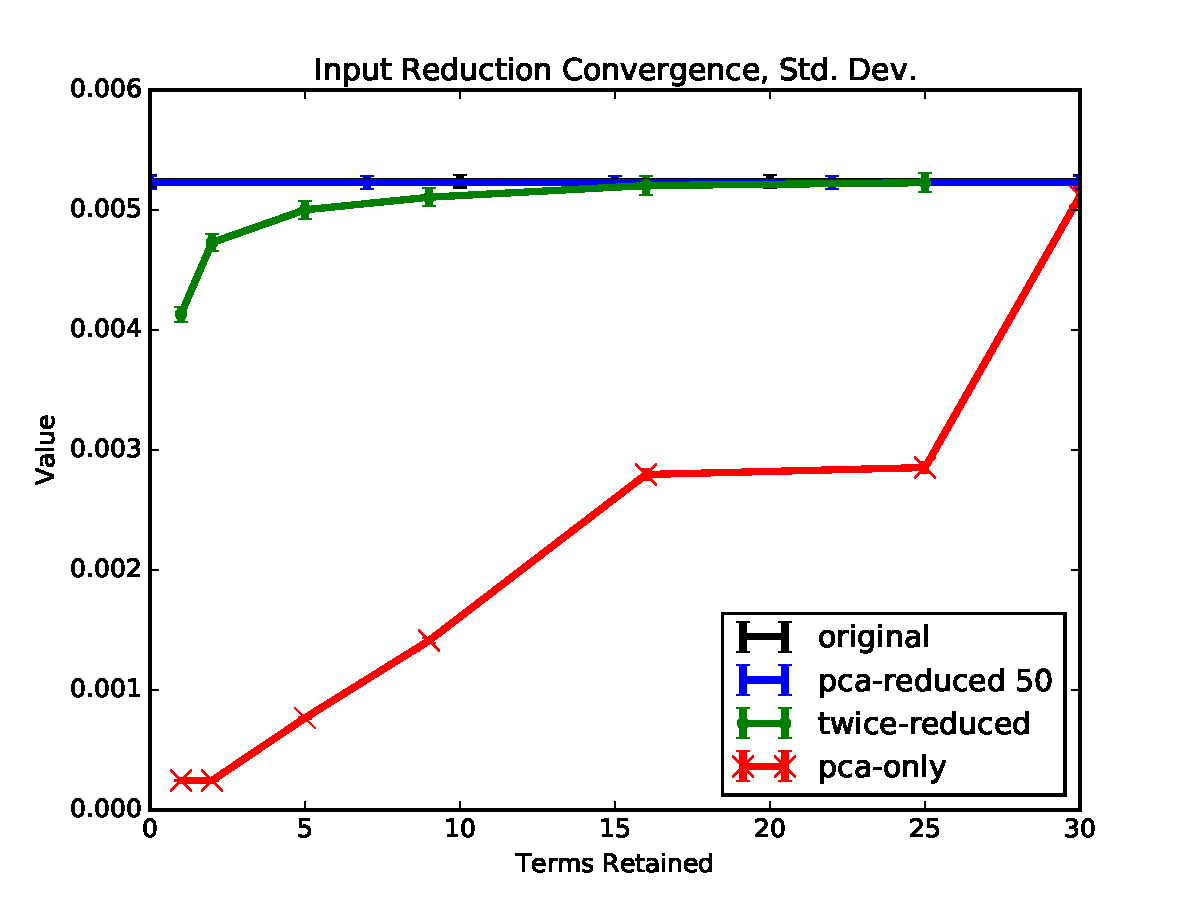
\includegraphics[width=\linewidth]{./example/first/var.pdf}
        \caption{Variance Values by Terms Kept}
      \end{figure}
    \end{column}
    \begin{column}{0.5\textwidth}
      \begin{figure}
        \centering
        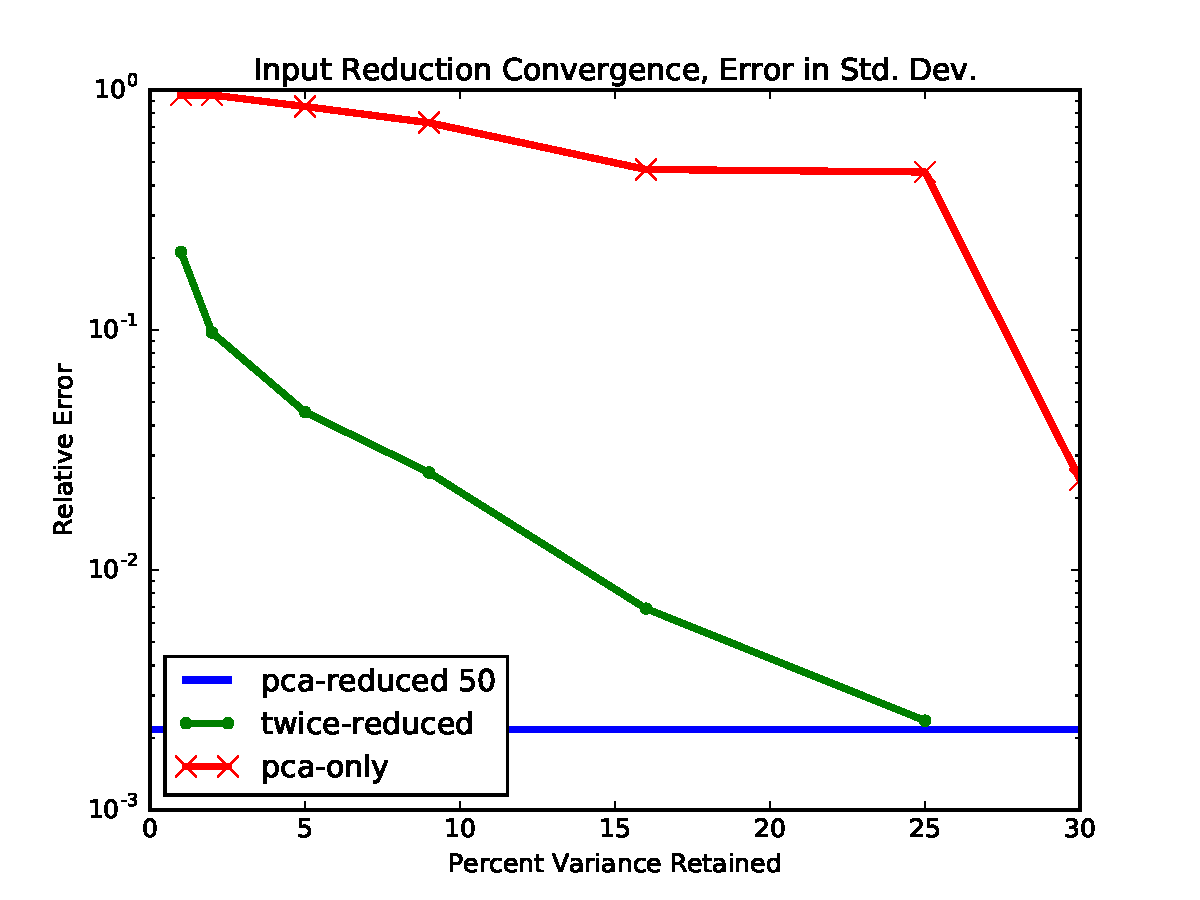
\includegraphics[width=\linewidth]{./example/first/var_err.pdf}
        \caption{Variance Errors by Terms Kept}
      \end{figure}
    \end{column}
  \end{columns}
\end{frame}

\begin{frame}[fragile]{Full Example: Number of Runs to Mean}
  \color{magenta} Monte Carlo (10k samples),
  \color{blue} Monte Carlo,
  \color{ForestGreen} Sparse Grid,
  \color{red} Adaptive Sobol
      \begin{figure}
        \centering
        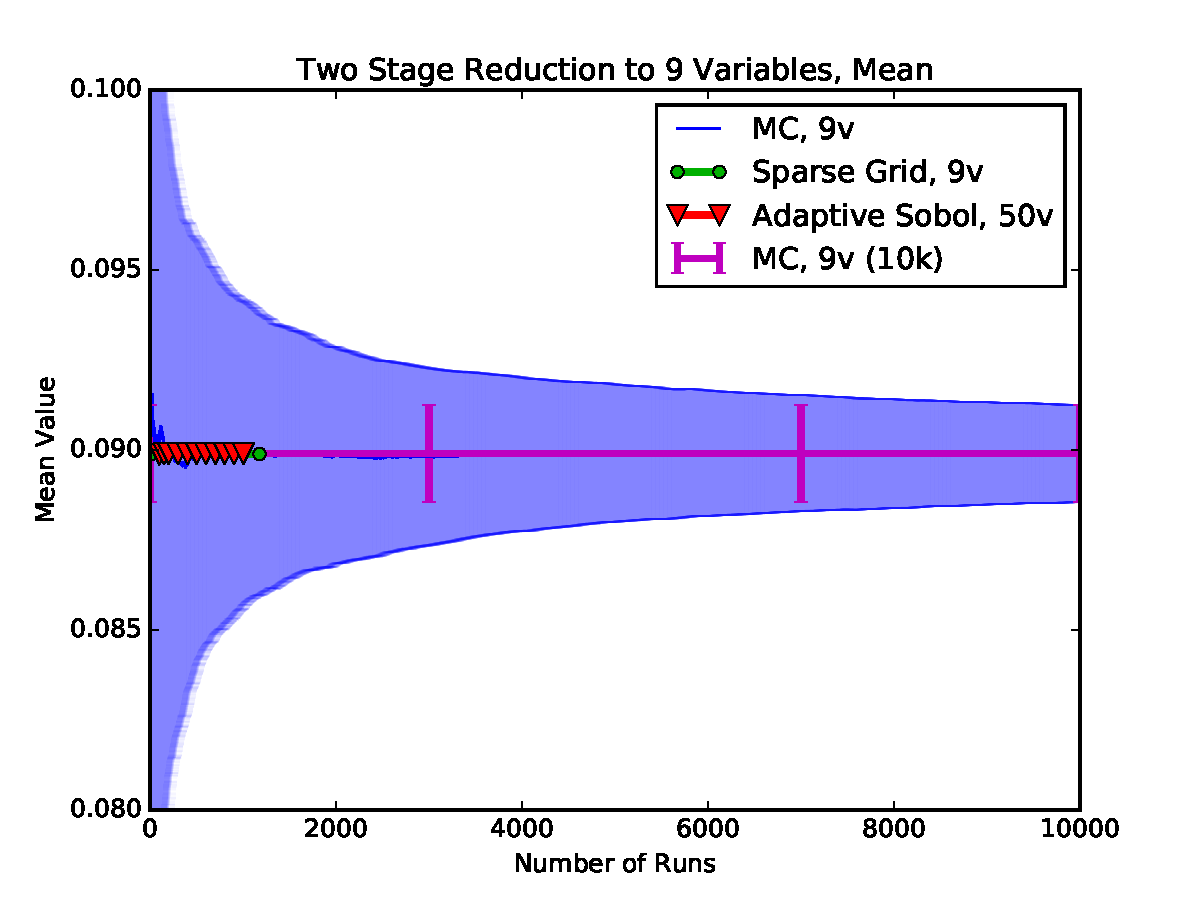
\includegraphics[width=0.7\linewidth]{./example/first/mc_vs_sc_mean_wide.pdf}
        \caption{Runs to Convergence, Mean, Twice-Reduced}
      \end{figure}
\end{frame}

\begin{frame}[fragile]{Full Example: Number of Runs to Mean}
  \color{magenta} Monte Carlo (10k samples),
  \color{blue} Monte Carlo,
  \color{ForestGreen} Sparse Grid,
  \color{red} Adaptive Sobol
      \begin{figure}
        \centering
        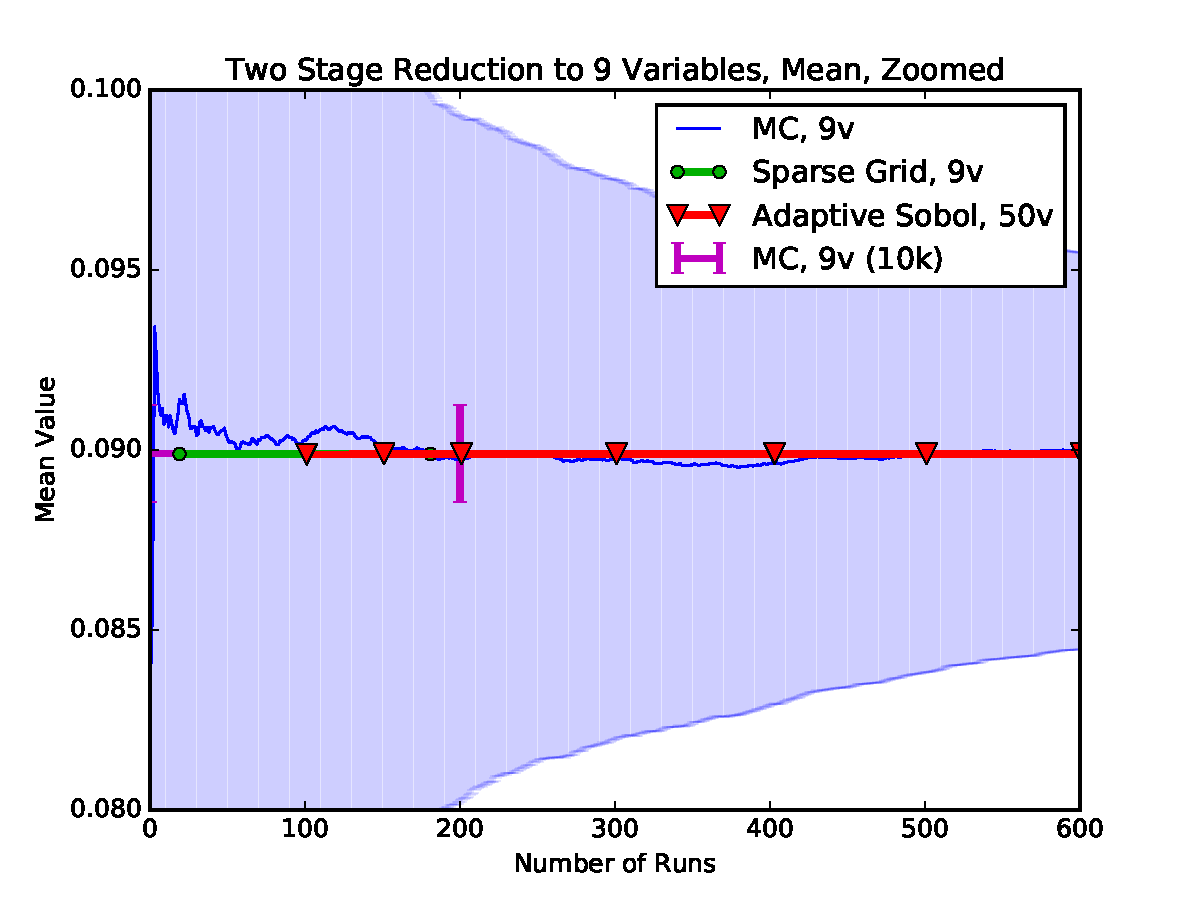
\includegraphics[width=0.7\linewidth]{./example/first/mc_vs_sc_mean.pdf}
        \caption{Runs to Convergence, Mean, Twice-Reduced}
      \end{figure}
\end{frame}

\begin{frame}[fragile]{Full Example: Number of Runs to Std. Dev.}
  \color{magenta} Monte Carlo (10k samples),
  \color{blue} Monte Carlo,
  \color{ForestGreen} Sparse Grid,
  \color{red} Adaptive Sobol
      \begin{figure}
        \centering
        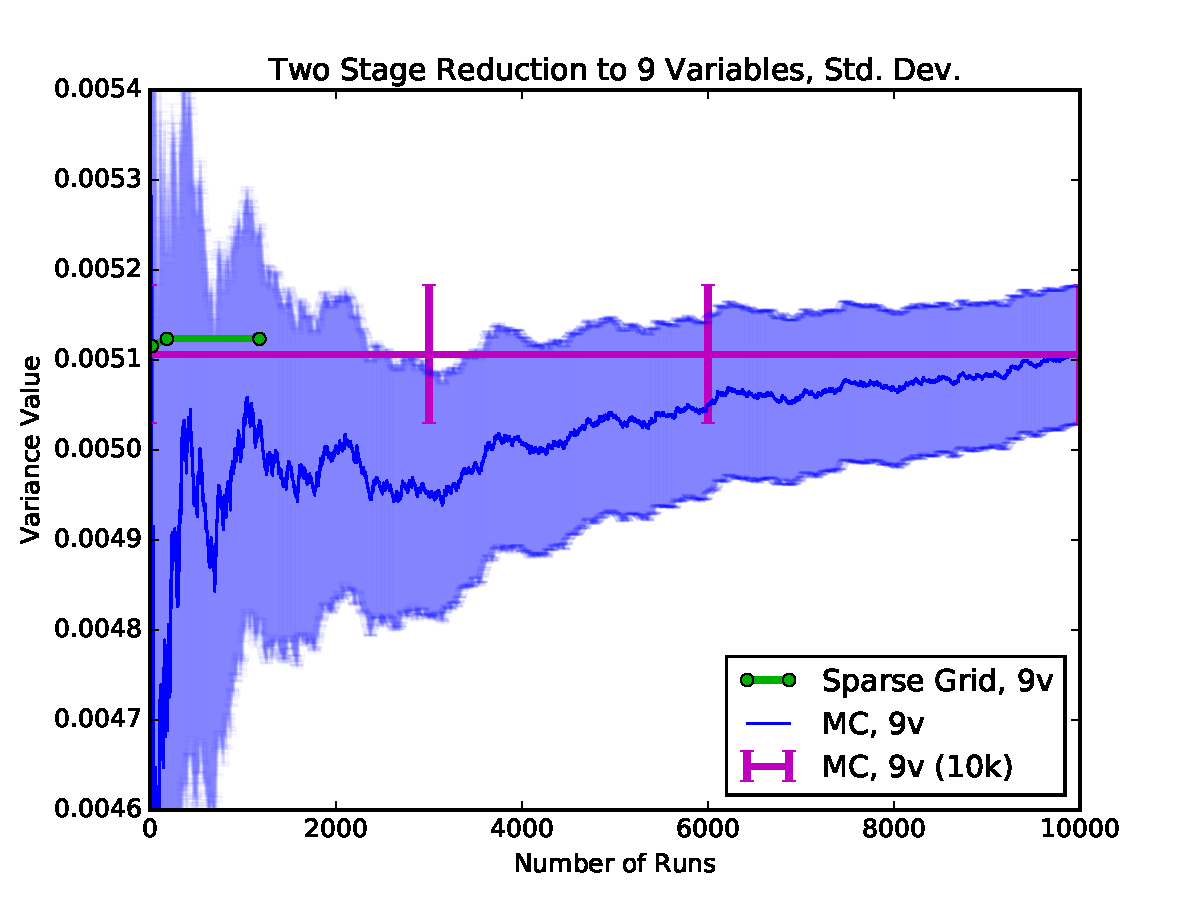
\includegraphics[width=0.7\linewidth]{./example/first/mc_vs_sc_var_wide.pdf}
        \caption{Runs to Convergence, Std. Dev., Twice-Reduced}
      \end{figure}
\end{frame}

\begin{frame}[fragile]{Full Example: Number of Runs to Std. Dev.}
  \color{magenta} Monte Carlo (10k samples),
  \color{blue} Monte Carlo,
  \color{ForestGreen} Sparse Grid,
  \color{red} Adaptive Sobol
      \begin{figure}
        \centering
        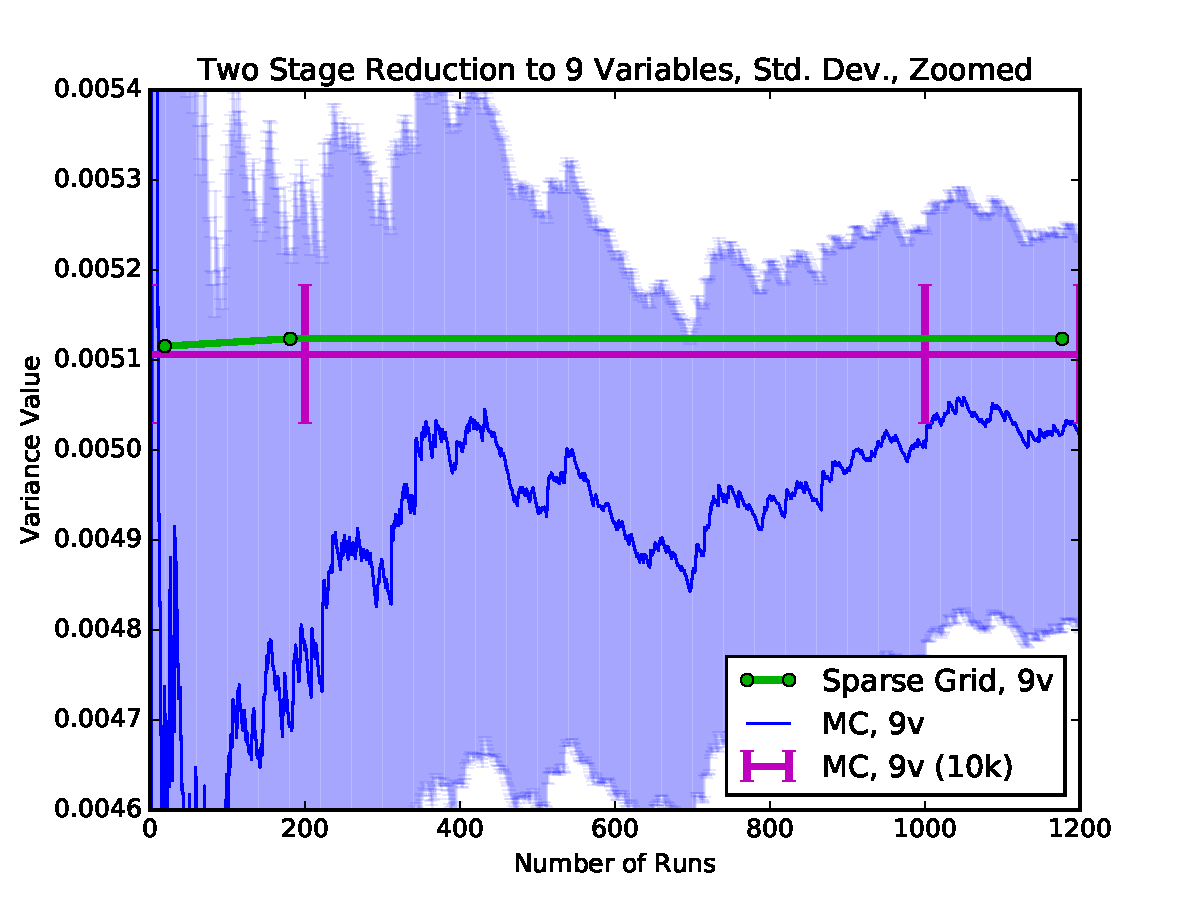
\includegraphics[width=0.7\linewidth]{./example/first/mc_vs_sc_var.pdf}
        \caption{Runs to Convergence, Std. Dev., Twice-Reduced}
      \end{figure}
\end{frame}

\begin{frame}[fragile]{Full Example: Convergence to Original Model}
  \color{magenta} Monte Carlo (10k samples),
  \color{blue} Monte Carlo,
  \color{ForestGreen} Sparse Grid,
  \color{red} Adaptive Sobol
      \begin{figure}
        \centering
        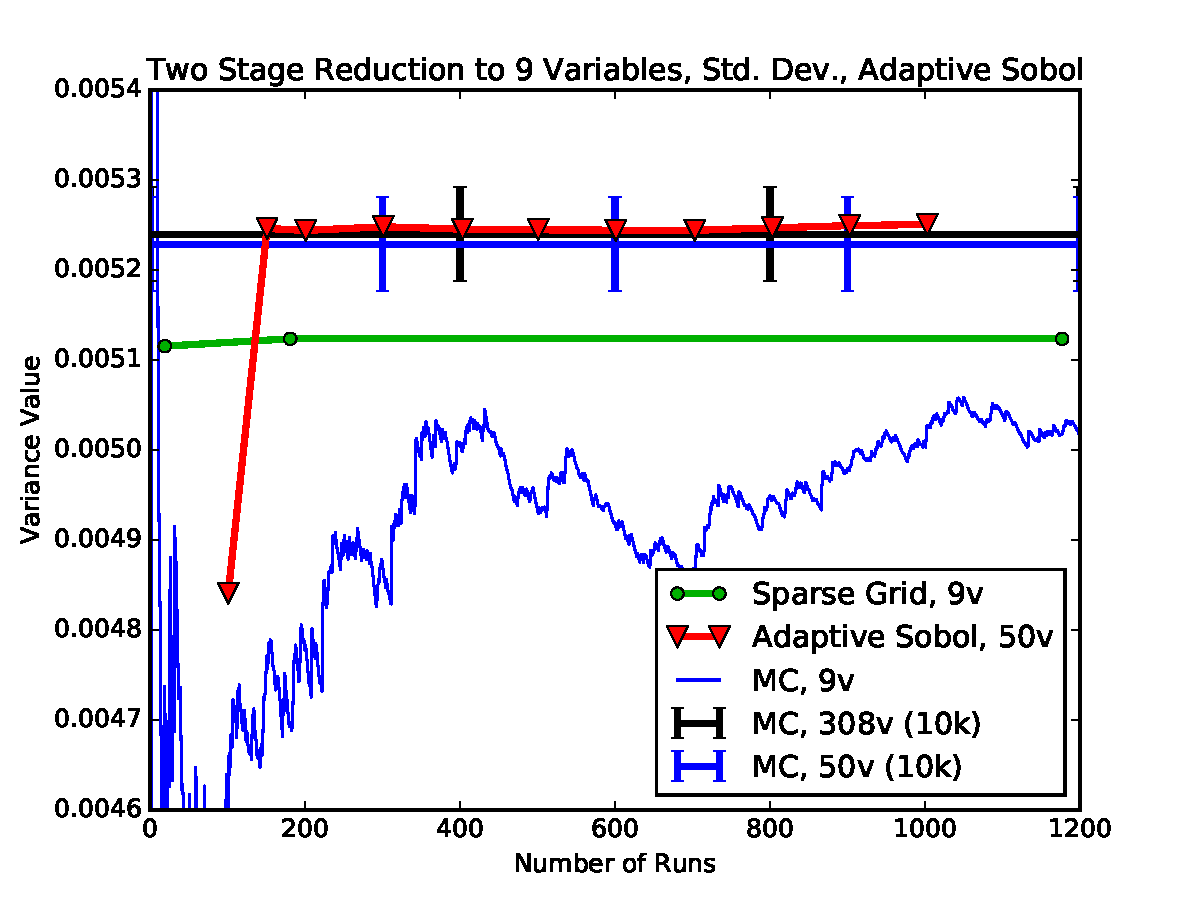
\includegraphics[width=0.7\linewidth]{./example/first/mc_vs_sc_var_adsob.pdf}
        \caption{Convergence to Original Model}
      \end{figure}
\end{frame}

\begin{frame}{End of Session}
\end{frame}



\end{document}

